\documentclass[a4paper,
fontsize=11pt,
%headings=small,
oneside,
numbers=noperiodatend,
parskip=half-,
bibliography=totoc,
final
]{scrartcl}

\usepackage[babel]{csquotes}
\usepackage{synttree}
\usepackage{graphicx}
\setkeys{Gin}{width=.6\textwidth} %default pics size

\graphicspath{{./plots/}}
\usepackage[ngerman]{babel}
\usepackage[T1]{fontenc}
%\usepackage{amsmath}
\usepackage[utf8x]{inputenc}
\usepackage [hyphens]{url}
\usepackage{booktabs} 
\usepackage[left=2.4cm,right=2.4cm,top=2.3cm,bottom=2cm,includeheadfoot]{geometry}
\usepackage{eurosym}
\usepackage{multirow}
\usepackage[ngerman]{varioref}
\setcapindent{1em}
\renewcommand{\labelitemi}{--}
\usepackage{paralist}
\usepackage{pdfpages}
\usepackage{lscape}
\usepackage{float}
\usepackage{acronym}
\usepackage{eurosym}
\usepackage{longtable,lscape}
\usepackage{mathpazo}
\usepackage[normalem]{ulem} %emphasize weiterhin kursiv
\usepackage[flushmargin,ragged]{footmisc} % left align footnote
\usepackage{ccicons} 
\setcapindent{0pt} % no indentation in captions

%%%% fancy LIBREAS URL color 
\usepackage{xcolor}
\definecolor{libreas}{RGB}{112,0,0}

\usepackage{listings}

\urlstyle{same}  % don't use monospace font for urls

\usepackage[fleqn]{amsmath}

%adjust fontsize for part

\usepackage{sectsty}
\partfont{\large}

%Das BibTeX-Zeichen mit \BibTeX setzen:
\def\symbol#1{\char #1\relax}
\def\bsl{{\tt\symbol{'134}}}
\def\BibTeX{{\rm B\kern-.05em{\sc i\kern-.025em b}\kern-.08em
    T\kern-.1667em\lower.7ex\hbox{E}\kern-.125emX}}

\usepackage{fancyhdr}
\fancyhf{}
\pagestyle{fancyplain}
\fancyhead[R]{\thepage}

% make sure bookmarks are created eventough sections are not numbered!
% uncommend if sections are numbered (bookmarks created by default)
\makeatletter
\renewcommand\@seccntformat[1]{}
\makeatother

% typo setup
\clubpenalty = 10000
\widowpenalty = 10000
\displaywidowpenalty = 10000

\usepackage{hyperxmp}
\usepackage[colorlinks, linkcolor=black,citecolor=black, urlcolor=libreas,
breaklinks= true,bookmarks=true,bookmarksopen=true]{hyperref}
\usepackage{breakurl}

%meta
%meta

\fancyhead[L]{Redaktion LIBREAS\\ %author
LIBREAS. Library Ideas, 38 (2020). % journal, issue, volume.
%\href{https://doi.org/10.18452/21547}{\color{black}https://doi.org/10.18452/21547}
{}} % doi 
\fancyhead[R]{\thepage} %page number
\fancyfoot[L] {\ccLogo \ccAttribution\ \href{https://creativecommons.org/licenses/by/4.0/}{\color{black}Creative Commons BY 4.0}}  %licence
\fancyfoot[R] {ISSN: 1860-7950}

\title{\LARGE{Editorial LIBREAS \#38: Tiere und Gewächse}}% title
\author{Redaktion LIBREAS} % author

\setcounter{page}{1}

\hypersetup{%
      pdftitle={Editorial LIBREAS \#38: Tiere und Gewächse},
      pdfauthor={Redaktion LIBREAS},
      pdfcopyright={CC BY 4.0 International},
      pdfsubject={LIBREAS. Library Ideas, 38 (2020).},
      pdfkeywords={Bibliothek, Flora und Fauna, Grüne Bewegung},
      pdflicenseurl={https://creativecommons.org/licenses/by/4.0/},
      pdfcontacturl={http://libreas.eu},
      pdflang={de},
      pdfmetalang={de}
     }



\date{}
\begin{document}

\maketitle
\thispagestyle{fancyplain} 

%abstracts

%body
\begin{quote}
\enquote{This is going to be a fantastic year for Britain.} (Boris
Johnson, 02. Januar 2020)
\end{quote}

Im Jahr 2020 haben wir gemeinsam viel gelernt. Einiges davon war
erstaunlich. Im März lernten wir zum Beispiel, dass es offenbar
notwendig ist, erwachsenen Menschen noch einmal beizubringen, wie man
sich richtig die Hände wäscht. Und, dass viele Menschen eher nur
ungefähr wissen (wussten), wie Immunsysteme und Ansteckungen
funktionieren oder wie man sich gesund hält. Aber damit ging es erst
los, denn es folgte ein direkt erlebbarer Kurs in Epidemiologie und
Gesundheitspolitik.

Was wissen wir heute nicht alles: Wie sich Viren vermehren und was sie
von Bakterien unterscheidet. Wie sich Viren verbreiten können. Was
Aerosole sind. Wo Aerosole sind. Dass es für den Stopp von
Viren-Übertragungen unterschiedlich effektive Masken gibt. Dass es
Masken gibt, die einen selbst schützen und dass es Masken gibt, die
andere schützen. Und dass beides nicht unbedingt dasselbe ist. Wir
lernten, dass die meisten Menschen versuchen, auf andere zu achten und
zu tun, was notwendig ist, um die Verbreitung von Krankheiten zu
vermindern. Wie lernten aber auch, dass dies einigen leichter und
anderen schwerer fällt. (Und dass es eine lautstarke Gruppe von Menschen
gibt, die sich dem aktiv verweigern.) Wir lernten, dass vieles in
unserer Lebenswelt nicht so eingerichtet ist, wie es aus hygienischen
Gesichtspunkten sinnvoll wäre. Was die Reproduktionszahl R ist und wie
sie berechnet wird. (Im Allgemeinen gab es ja nebenher 2020 auch noch
einen Auffrischungskurs in Mathematik.) Dass Viren gar keine Lebewesen
sind und somit auch nicht sterben können.

Wir konnten auch live erleben, wie sich wissenschaftliches Wissen
fortentwickelt und wie es in Politik und Gesellschaft interpretiert
wurde. Nicht zuletzt kennen wir jetzt solche Einrichtungen wie das
Robert-Koch-Institut in Berlin, das Bundesamt für Gesundheit in
Liebefeld und das Statens Serum Institut im Artillerivej in Kopenhagen
und wissen, wer grundsätzlich für die Gesundheitspolitik in den Staaten,
Ländern und Kantonen zuständig ist, in denen wir leben. Wer hätte im
Januar 2020 geahnt, dass wir in diesem Jahr Spezialwissen solcher Art
erwerben? Es war in der Tat ein Wissenschaftsjahr und plötzlich fanden
sich auf den Nachtschränken Bücher wie \enquote{Epidemiologie für
Dummies} (Razum, Oliver; Breckenkamp, Jürgen; Brzoska, Patrick. 3.
Aufl., 2017).

\begin{figure}
\centering
\includegraphics{img/redaktionsorte.png}
\caption{Redaktionsorte XVII. Online, Oktober 2020}
\end{figure}

Wir wussten nicht, was dieses Jahr alles an Lerneffekten bringen würde,
als wir das Thema \enquote{Tiere und Gewächse} konzipierten. Tatsächlich
hatten wir erwartet, in den Texten einer ganzen Reihe von
Mikroorganismen zu begegnen, aber vor allem im Bezug auf den
Bestandserhalt. Dazu gibt es dann tatsächlich auch Texte in der Ausgabe.
Unsere Vorstellung, dass das Thema auch viele Einblicke in den Alltag
der Bibliotheksarbeit, in Büros und Nutzungszonen, Magazine und Orte wie
\emph{Urban Gardens}, liefern würde, schlug sich leider nur in einigen,
kurzen Artikeln nieder. Die Bibliothekswelt ist vielleicht grün. Aber
offenbar schreibt sie nicht so gern darüber.

Das Erstellen dieser Ausgabe fühlte sich wie die \enquote{echte}
Pandemie-Ausgabe an: Alle hatten noch mehr zu tun als sonst schon.
Vieles war in Veränderung. Alltag war nur wenig normal. Vielleicht kamen
deshalb nicht so viele Beiträge zum Themenschwerpunkt zusammen, wie wir
uns erhofften. Aber die, die wir erhalten haben, sind interessant, auch
weil sie oft andere Formen wählten als den wissenschaftlichen Artikel.

Die Pandemie hat uns alle überrollt. Was wir allerdings schon Anfang
2020 (und weit früher) wussten, ist, \emph{dass die Klimakatastrophe die
Gesellschaften noch viel stärker überrollen wird}. Krise als Chance --
das wäre etwas gewesen. Die kurzzeitig dank Lockdown-Maßnahmen
zurückgehenden Emissionen waren ein bemerkenswerter Nebeneffekt. Er hat
sich längst wieder in Rauch aufgelöst (leider, sofern es einer solchen
Kommentierung überhaupt bedarf). Die Maschine der Wirtschaft läuft
weiter, in den USA und am Amazonas verbrennen die Wälder und schaffen es
nur noch bestenfalls auf die Seite Vermischtes der Tageszeitungen.
Deutschland setzt neuerdings wieder auf Autobahnausbau und sehnt sich
nach dem Trugbild einer weiterhin permanent wachsenden Leistungs- und
Konsumgesellschaft. In der Schweiz planen viele Menschen, so Umfragen,
nach der Pandemie mehr zu fliegen und zu kaufen, als schon vor der
Pandemie. Es ist nicht leicht, in diesen Zeiten Optimist*in zu sein.
Aber es gibt trotz allem Hoffnungszeichen. In den letzten Jahren begann
eine neue Generation von Aktiven, diese Katastrophe wieder auf die
politische und gesellschaftliche Tagesordnung zu zwingen. Der Elan der
\enquote{Klimajugend} hat -- was notwendig ist -- viel in Aufbruch
gesetzt. Auch Bibliotheken. Im Jahr 2019 wurde deshalb, unter anderem
mit Unterstützung durch den LIBREAS.Verein, Libraries4Future gegründet.

Wir wollen weiter unseren Beitrag dazu leisten, das Thema
voranzutreiben: Die Pandemie wird irgendwann vorbei oder wenigstens
gezähmt sein und uns unter anderem neues Wissen hinterlassen. Die
Klimakatastrophe kommt und wir entscheiden, wie sehr wir sie weiter
zuspitzen wollen und wo wir sie eventuell noch etwas abmildern können.
Ein Jahr nach der Gründung von Libraries4Future haben wir deshalb zu
einem zweiten Schwerpunkt eingeladen, der die tatsächlichen Aktivitäten
von Bibliotheken in diesem Bereich beleuchten soll. Es ist, wie wir auch
2020 noch einmal handfest erleben durften, nicht die einzige Baustelle,
vor der die ganze Welt steht. Es sei nur daran erinnert, dass im Zuge
der Black-Lives-Matters-Proteste im Sommer 2020 auch im Bereich von
Rassismus und seinen Strukturen in unseren Gesellschaften einiges
gelernt, aber leider noch nicht viel verändert wurde. Die Sorge um die
physischen Lebensgrundlagen auf unserem Planet ist jedoch naturgemäß
aber eine der drängendsten.

2020 fühlte sich an, wie die oft kaum mehr erträgliche Zuspitzung von
Entwicklungen, die man hätte sehen können -- die man aber oft zur Seite
schob. Das funktioniert aber nur solange, bis es einen einholt. Im
Oktober 2020 blühen die Kastanienbäume, weil sie so beschädigt sind,
dass sie sterben werden. Es ist ein letztes Aufbäumen. Die Zeitung
schreibt, dass wir in Städten und Wäldern neue Arten von Bäumen
brauchen, die robuster sind, um die Dauerdürren in Europa zu ertragen.
Wir haben wirklich viel gelernt in diesem Jahr, weil man aus jeder
Katastrophe viel lernt. Vor allem sehen wir noch besser als zuvor, was
auf dem Spiel steht. Was wir tun können und werden, wird uns in Zukunft
begleiten. Man ist nie zu alt für diese Art Coming-of-Age.

\begin{figure}
\centering
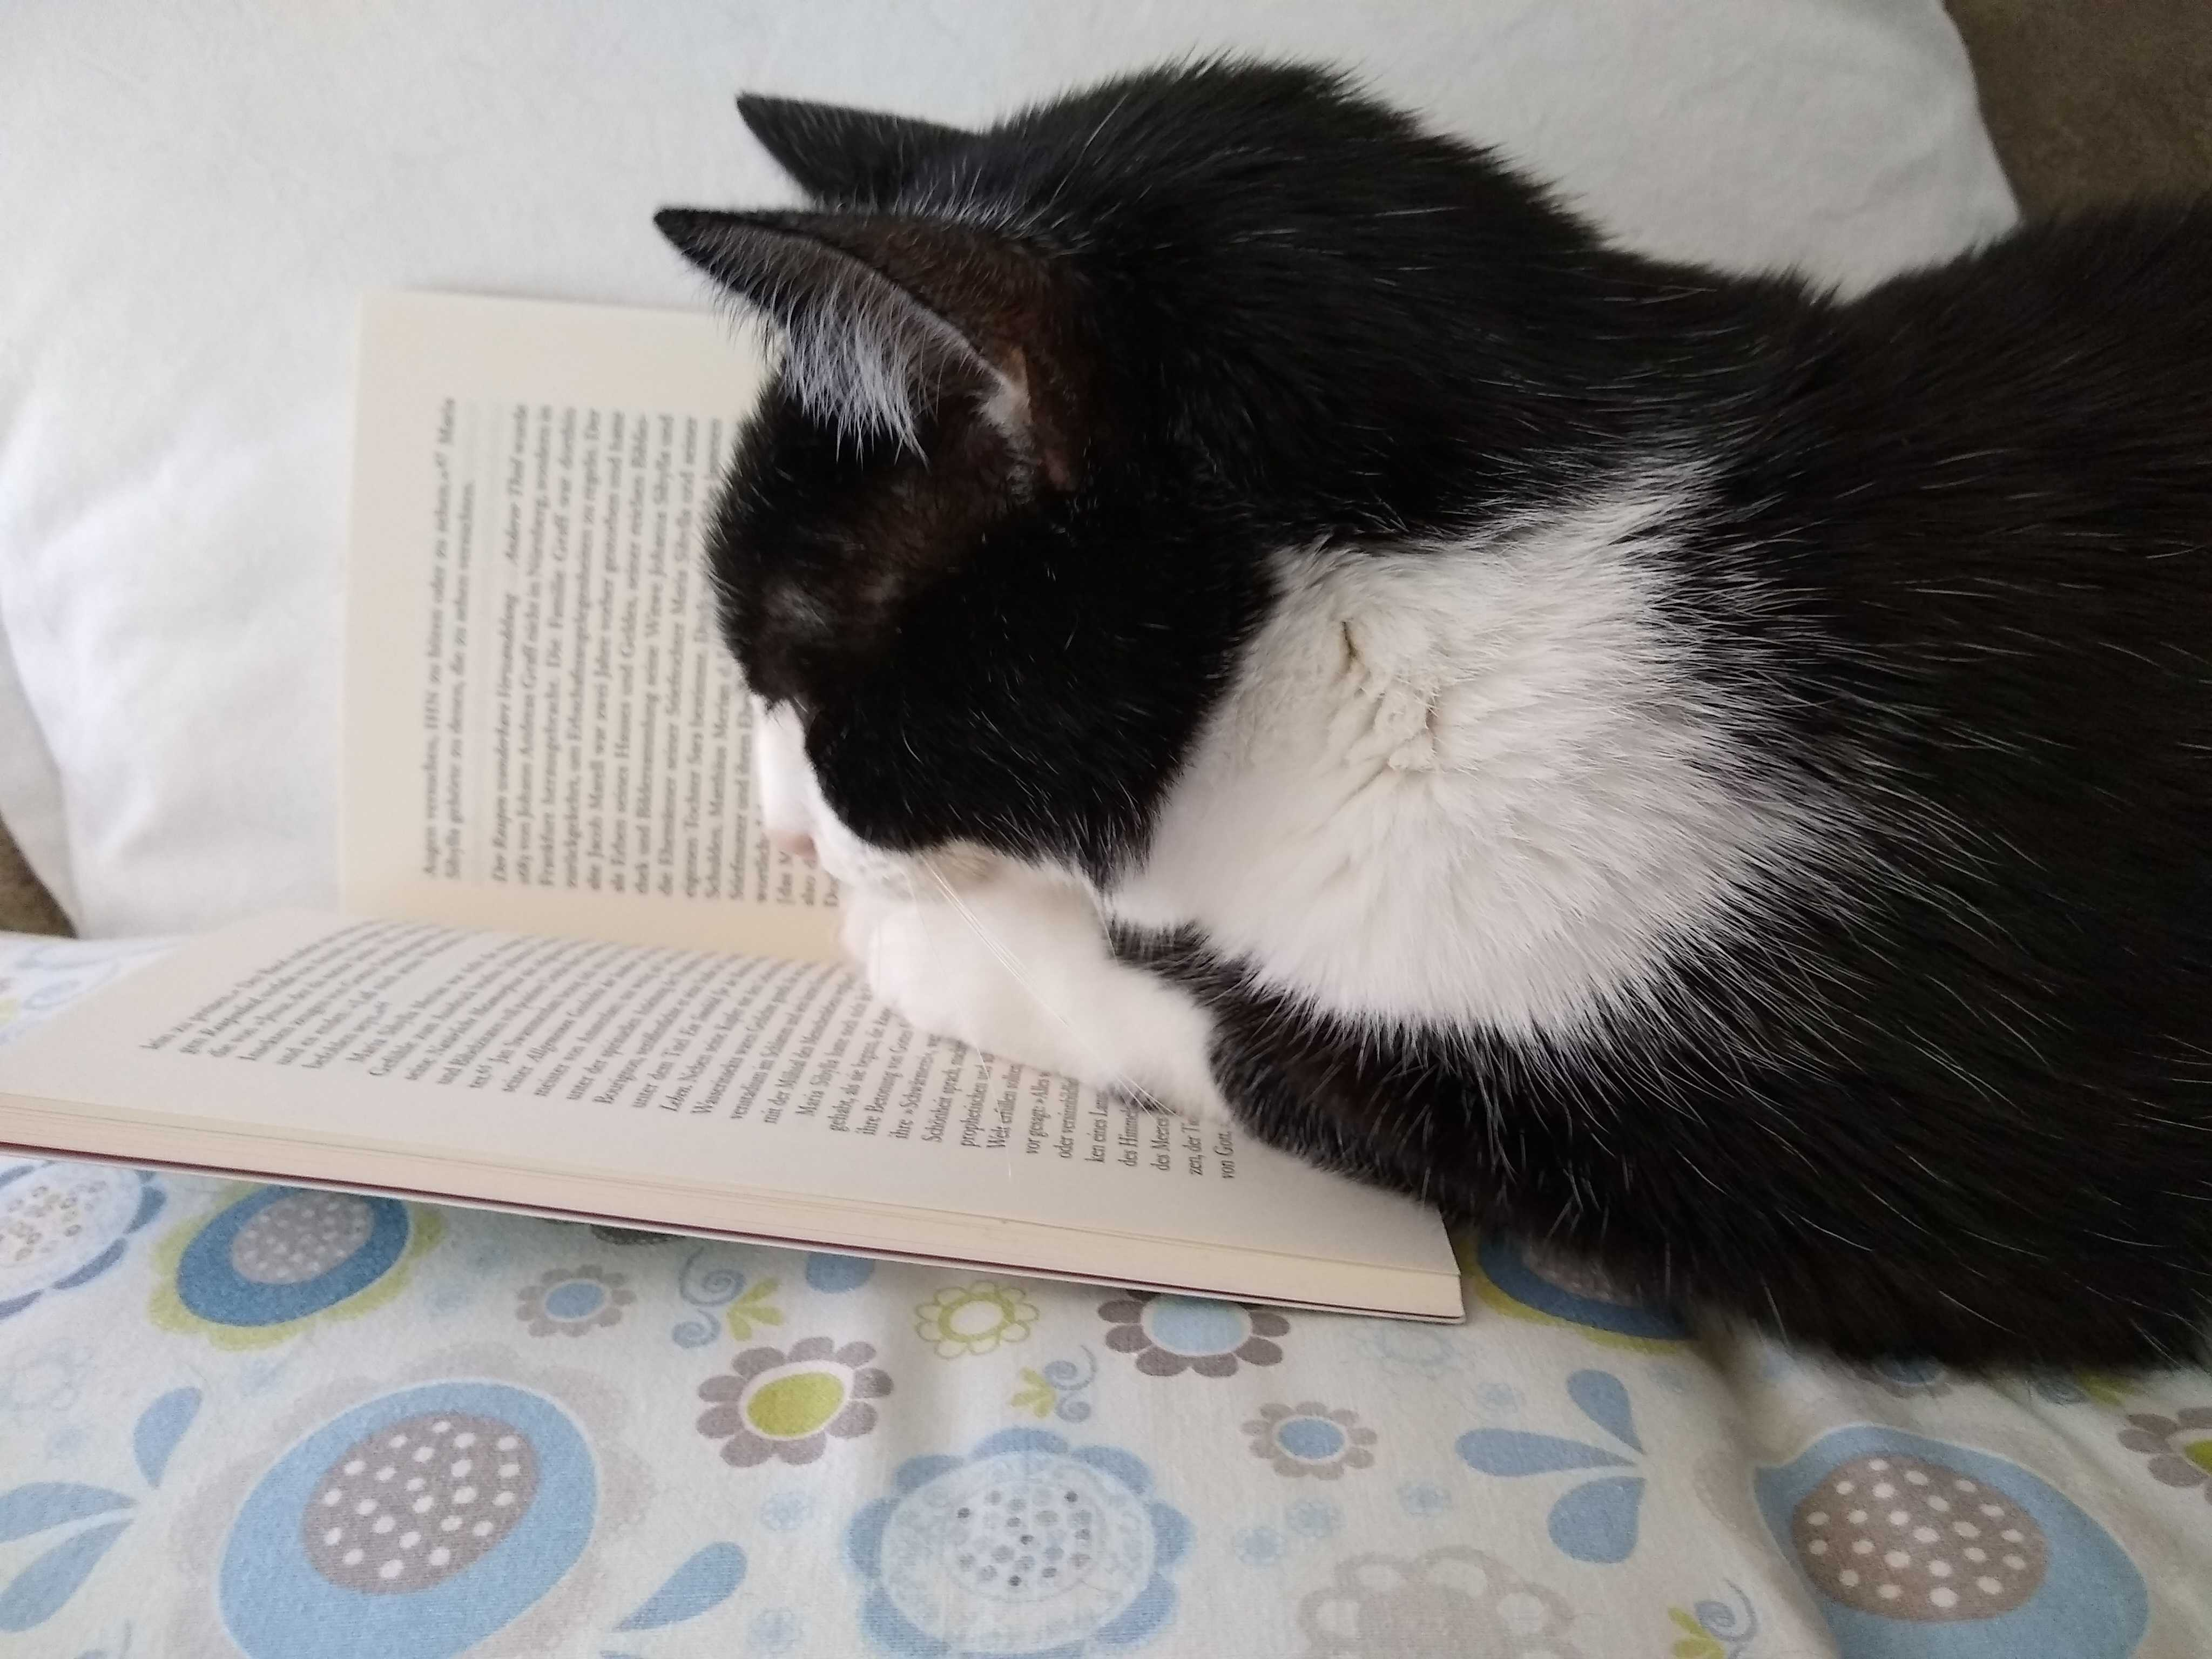
\includegraphics{img/felix-liest.jpg}
\caption{LIBREAS-Redaktionskatze Felix liest: Wulf, Andrea (2012): Die
Jagd auf die Venus. Bertelsmann, 320 Seiten. ISBN: 9783570100950}
\end{figure}

Im Redaktions-Chat werden, wie sollte es auch anders sein, regelmäßig
auch Fotos, Texte und Nachrichten zu Tieren geteilt (Pflanzen kommt
bisher vergleichsweise wenig Aufmerksamkeit zu). Bibliotheken spielen
dabei seltener eine Rolle -- Kuriosa und Erheiterung stehen im
Vordergrund. Manchmal sind es auch Zeugnisse davon, wie Haustiere zu
Arbeitsverhinderern werden können. Fast schon auf natürliche Weise kamen
wir so zur Frage des Lieblingstiers, deren Ergebnis überraschen mag
(zumindest wenn man dem Stereotyp der Katzen zugeneigten Bibliothekar*in
glauben darf). In der Redaktion dieser Ausgabe:

\begin{itemize}
\tightlist
\item
  Team Hund, 3 Mal
\item
  Team Katze, 2 Mal
\item
  Team Eichhörnchen, 1 Mal
\item
  Team Eule, 1 Mal
\item
  Team Igel, 1 Mal
\end{itemize}


Unterdessen ist LIBREAS. Library Ideas nun gerade erst -- oder schon --
15 Jahre alt geworden. Wir hatten geplant, das größer zu begehen -- aber
Covid und eine Flut der allgemeinen Unsicherheit kam dazwischen. Wir
hoffen, es zum 16. Jahrestag nachholen zu können.

Anlässlich dieses Geburtstages hat die Redaktion ein Buch
zusammengestellt, in dem sie Lieblingstexte aus diesen 15 Jahren LIBREAS
versammelt hat. Es ist eine Übersicht und Bestandsaufnahme zugleich. Ein
Rückblick mit einem gewissen Stolz, all die Jahre eine Zeitschrift
produziert zu haben, die wir gerne lesen würden. Was nicht ohne unsere
Autor*innen und Leser*innen möglich gewesen wäre.

Dafür unseren besten Dank.

Eure / Ihre Redaktion LIBREAS. Library Ideas

(Aarhus, Berlin, Hannover, Lausanne, München)

%autor

\end{document}
